\documentclass[tikz,border=10pt]{standalone}
\usepackage{tikz}
\usetikzlibrary{arrows, calc, positioning}

\definecolor{myDeepBlue}{RGB}{0, 40, 75}
\definecolor{myBlue}{RGB}{98, 196, 221}
\definecolor{myRed}{RGB}{233, 75, 87}

\tikzstyle{box}= [draw=myDeepBlue, line width=0.5mm,rounded corners=0.5mm]
\tikzstyle{Box}= [minimum width=1.5cm, minimum height=0.75cm, box]

\begin{document}
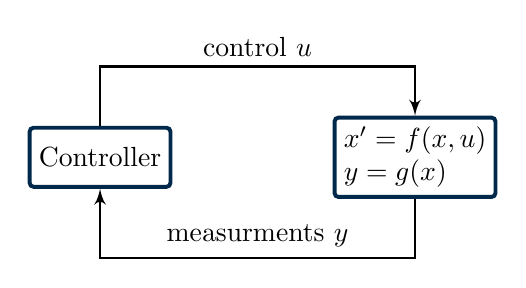
\begin{tikzpicture}[node distance=2cm,auto,>=latex']
    % Define a distance variable
    \pgfmathsetmacro{\mydist}{4cm}

    \node [Box] (Controller) {Controller};
    \node [Box, right of=Controller, node distance=\mydist, align=left] (System)
    {$x' = f(x,u)$ \\
    $y = g(x)$};

    % action path
    \draw[->, line width=1pt] (Controller.north)
    -| ++(0,0.75)
    -| (System.north) node[near start, above] {control $u$};

    % observation path
    \draw[->, line width=1pt] (System.south)
    -| ++(0,-0.75)
    -| (Controller.south) node[near start, above] {measurments $y$};

\end{tikzpicture}
\end{document}